\documentclass[convert={density=900,size=1080x800,outext=.png}]{standalone}
\usepackage{tikz}

\usetikzlibrary{calc, positioning}
\usetikzlibrary{arrows.meta}
\usetikzlibrary{matrix}
\usetikzlibrary{shadows}
\usepgflibrary{shapes.misc}
\usepgflibrary{{shapes.geometric}}

\pgfdeclarelayer{shadow} 
\pgfsetlayers{shadow,main}
\def\shadowradius{3pt}


\def\mw{1.25cm}
\def\mh{1cm}

\tikzstyle{component} = [draw, fill=white, minimum width=\mw, minimum height=\mh, align=center]

\tikzset{
    border/.style = { 
        draw, rectangle, minimum width=\mw, minimum height=\mh, thick, align=center, ultra thick
    },
    Component/.pic = {
        \node [border](-edge){#1}; 
    },
}

\tikzset{
    clockborder/.style = { 
        trapezium, trapezium angle=60, minimum width=1cm, draw, very thick
    },
    Clock/.pic = {
        \node [clockborder, shape border rotate=-180](-clockedge){#1};
        \draw[very thick] (-clockedge.east) -- ++(2cm, 0cm);
        \def\sft{0.5}
        \foreach \x in {0, 0.5, 1, 1.5}{
            \draw[very thick] (\x + \sft, 0.1) -| ++(0.25cm, 0.25cm) -| ++ (0.25cm, -0.25cm);
        }
    },
}

\begin{document}
    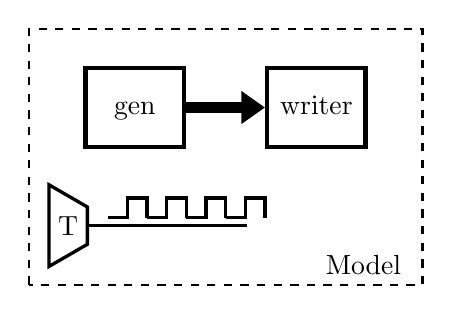
\begin{tikzpicture}
        % Place the blocks 
        \matrix (m) [
            matrix of nodes, 
            ampersand replacement=\&, 
            column sep = 1cm, 
            row sep = 1cm, 
            nodes={
                text height=1.5ex,
                text depth=.25ex,
                anchor=center}
                ]{
                    \draw pic (gen) {Component={gen}}; \& \draw pic (writer) {Component={writer}}; \\
                };

        % Draw connections 
        \begin{scope}[line width=1.5mm, >={Triangle[width=4mm,length=3mm]}]
            \def\shiftamount{0.5mm};
            \draw[->] (gen-edge.east) -- (writer-edge.west);
        \end{scope}

        % \Place clock 
        \begin{scope}[shift={(-2cm, -1.5cm)}]
            \draw pic(clk) {Clock={T}} ;
        \end{scope}

        %  Draw rectangle 
        \draw[dashed, thick] (-2.5, -2.25) rectangle (2.5, 1);
        \draw (0,0) node[yshift=-2cm, xshift=1.75cm]{Model};
    \end{tikzpicture}
\end{document}